\documentclass[12pt]{article}
\usepackage{coursenote}

\begin{document}
\title{STAT 401 Chapter 1}
\maketitle

\section{Relations between variables}

\subsection{Functional relation: $y = f(x)$}

\indentblock{Data points $(x_i, y_i)$ fall exactly on the function
curve.}

\subsection{Statistical relation: $y = f(x) + \epsilon$}

\indentblock{For any fixed value $x$,
$Y$ has a random scatter, or fluctuation, about the
deterministic function $f(x)$.}

\bigskip

\example
\begin{enumerate}
\item $Y$ = \% body fat, $X$ = age.
\item
    $Y$ = cases of beer sold at the liquor store on a given Saturday,
    $X$ = number of college basketball games being aired that weekend.
\item
    $Y$ = number of snow shovels sold in a given week,
    $X$ = average daily temperature for that week.
\item
    $Y$ = number of miles driven per year, $X$ = urban/rural driver.
\item
    $Y$ = change in cholesterol level,
    $X$ = placebo vs.\ active drug treatment group.
\item
    $Y$ = direction from beehive at which bee disappears from sight,
    $X$ = species of bee.
\item $Y$ = actual fish length, $X$ = length as recorded by sonar.
\end{enumerate}

In this course we work with quantitative or qualitative (\ie
categorical) $X$, and quantitative $Y$.
We do not work with qualitative $Y$.

\subsection{Types of studies}

\emph{Observational}

\emph{Experimental}

Observational study: may deduce correlation, but \emph{not} causation.

Well-designed, well-run experimental study: may deduce causation.

\section{Least squares (LS) estimation}
\label{sec:ls}

\textsf{Example data set} Mazda Price data: asking prices (Australian dollars) for 124 Mazda
cars, along with the age of the car (years). (Reprinted in Data
Analysis: An Introduction Based on R, by A.~Lee, Auckland: Department of
Statistics, University of Auckland.)

\begin{figure}
(a)
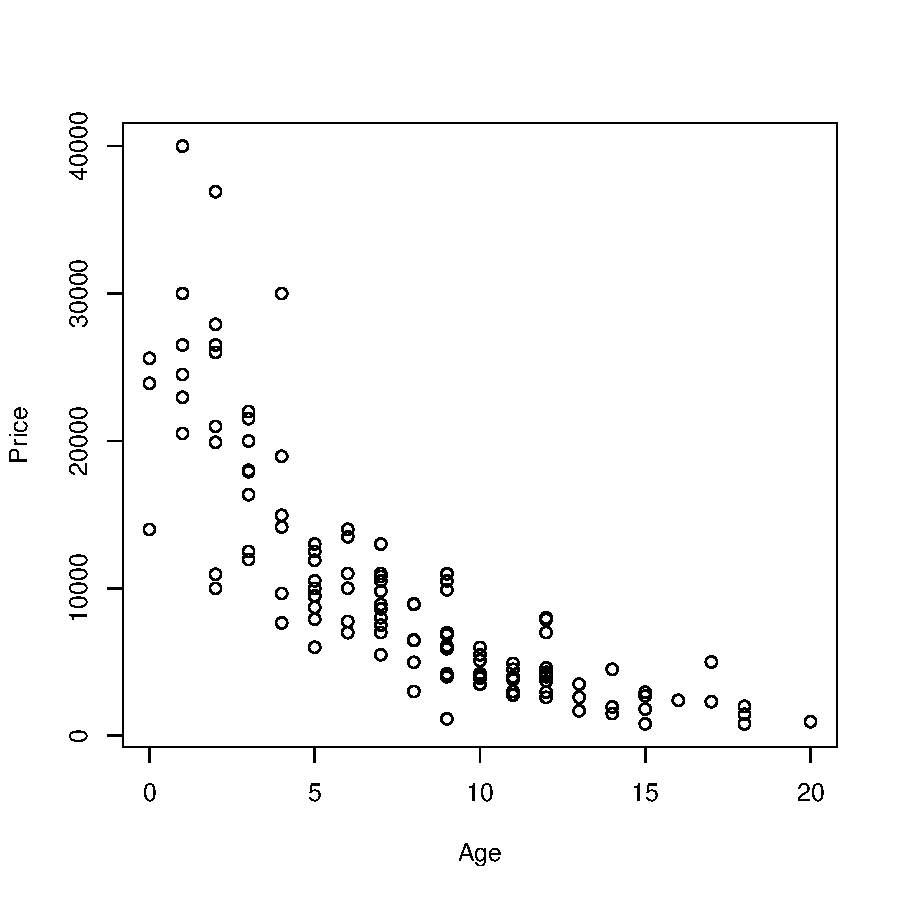
\includegraphics[width=.42\textwidth]{fig_mazda_raw.pdf}
(b)
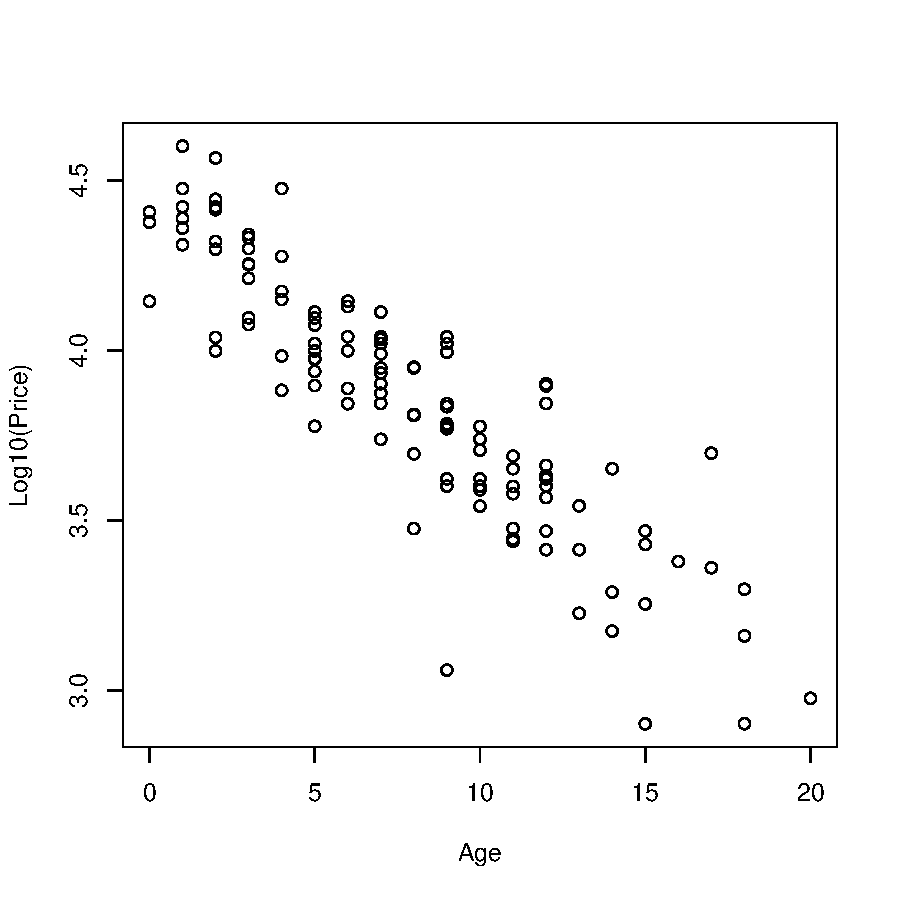
\includegraphics[width=.42\textwidth]{fig_mazda_log_transformed.pdf}
\caption{Mazda data. (a) Original. (b) Log transformed.}
\label{fig:mazda-data}
\end{figure}

Apparently there exists some relation between age and price.
The relation is statistical because at a certain age,
the price is not uniquely determined.

The relation does not appear to be linear.
We log-transform the price, then
\mbox{$\log_{10}(\text{price}) \sim \text{age}$}
looks like linear.
So we take age as $X$ and $\log_{10}(\text{price})$ as $Y$.

\emph{Suppose} a \emph{linear} relation is a good description
for this relationship:
\[
Y_i = \beta_0 + \beta_1 X_i + \epsilon_i
,
\]
where $\beta_0$ is intercept
and $\beta_1$ is slope.
They are both regression coefficients.
But they are unknown and need to be estimated from the data.

What are the values of $\beta_0$ and $\beta_1$?
In other words, we want to find (or ``estimate'')
a function $y = b_0 + b_1 x$ that is the ``best fit'' to this dataset.
(Apparently we can't find a ``perfect'' fit.)

What is the criterion for a ``good fit''?

The \emph{least squares} criterion:
the best fit is given by $\beta_0$ and $\beta_1$ that
minimize the following quantity:
\[
Q = \sum_{i=1}^n (Y_i - \beta_0 - \beta_1 X_i)^2.
\]
This is the most commonly used criterion for ``best fit'',
and it makes intuitive sense.
In words, we find $\beta_0$ and $\beta_1$ values that minimize
the \emph{total squared distances}
between the fitted values (\ie $\beta_0 + \beta_1 X_i$)
and the observed values (\ie $Y_i$).

Denote the solutions by $\hat{\beta_0}$ and $\hat{\beta_1}$.
They are found by setting
$\frac{\partial Q}{\partial \beta_0} = 0$ and
$\frac{\partial Q}{\partial \beta_1} = 0$,
that is,
\begin{align}
\frac{\partial Q}{\partial \beta_0}
&= \sum 2(Y_i - \beta_0 - \beta_1X_i)(-1)  = 0\\
\frac{\partial Q}{\partial \beta_1}
&= \sum 2(Y_i - \beta_0 - \beta_1X_i)(-X_i) = 0
\end{align}
This leads to
\begin{equation}\label{eq:normal-eqn}
\begin{split}
\sum Y_i &= n \hat{\beta_0} + \hat{\beta_1} \sum X_i, \\
\sum X_i Y_i &= \hat{\beta_0} \sum X_i + \hat{\beta_1} \sum X_i^2.
\end{split}
\end{equation}
%This system of equations is called the ``normal equations''.
Its solution is
\begin{equation}\label{eq:LS}
\hat{\beta_1}
=
    \frac{\sum \bigl(X_i - \overline{X}\bigr)
        \bigl(Y_i - \overline{Y}\bigr)}
    {\sum \bigl(X_i - \overline{X}\bigr)^2}
= \frac{S_{xy}}{S_{xx}}
,\quad
\hat{\beta_0} = \overline{Y} - \hat{\beta_1} \overline{X}
.
\end{equation}
This gives formulas for estimating the regression coefficients
using the available data $(x_1, y_1),\dotsc, (x_n,y_n)$.

With the Mazda data, we find\\
\hspace*{1cm}$n = 24$,\\
\hspace*{1cm}$\sum X_i = 964$,\ \  $\sum Y_i = 479.69$,\\
\hspace*{1cm}$\sum X_i^2 = 10138$,\ \  $\sum Y_i^2 = 1872.67$,\\
\hspace*{1cm}$\sum X_iY_i = 3540.09$.\\
The LS estimates of the slope and intercept are
$b_1 = -0.0715$ and $b_0 = 4.4245$, respectively.

\begin{figure}
\begin{center}
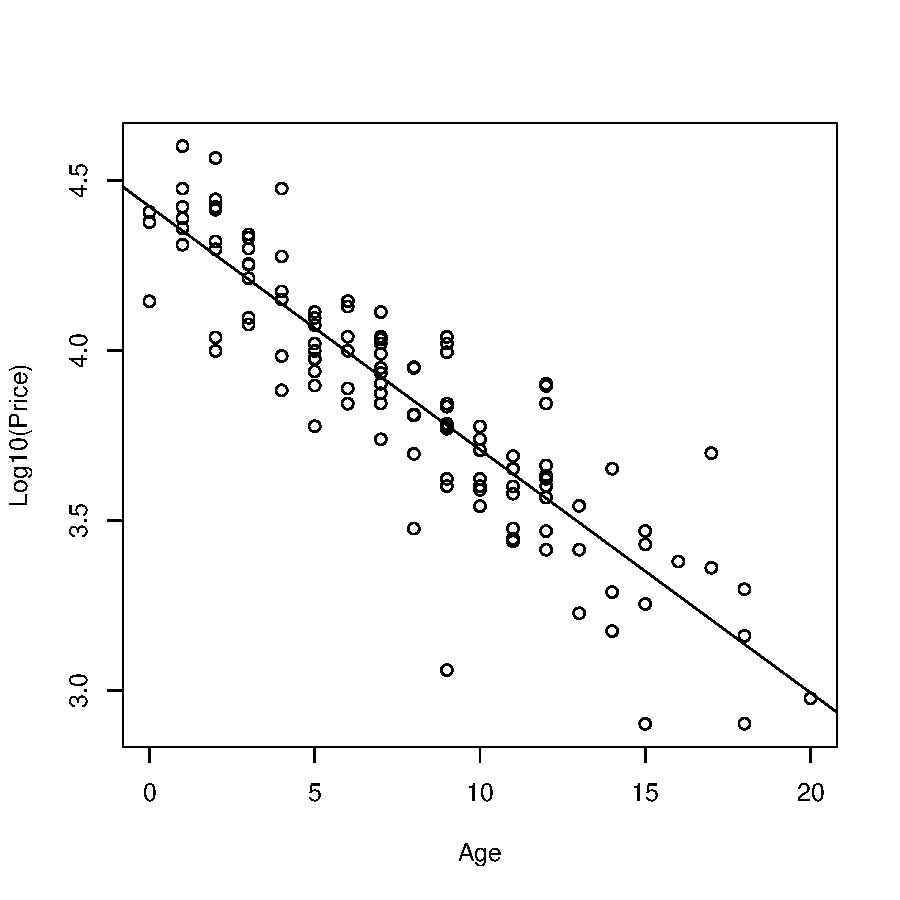
\includegraphics[width=.5\textwidth]{fig_mazda_log_fit.pdf}
\caption{Mazda data: fitted model}
\label{fig:mazda-fitted}
\end{center}
\end{figure}

$\hat{\beta_0}$ and $\hat{\beta_1}$ are called ``estimators''
(\ie formulas for calculating estimates).

$b_0$ and $b_1$ are called ``estimates''
(\ie actual values based on actual data).

\hrulefill

An oft-used re-formatting:
\[\begin{split}
\sum(X_i - \overline{X})(Y_i - \overline{Y})
&= \sum \bigl(X_iY_i - X_i\overline{Y} - \overline{X}Y_i +
    \overline{X}\overline{Y}\bigr)
\\
&= \sum X_iY_i - \frac{\sum Y_i}{n} \sum X_i
    - \frac{\sum X_i}{n} \sum Y_i
    + n\frac{\sum X_i}{n} \frac{\sum Y_i}{n}
\\
&= \sum X_iY_i - \frac{1}{n}\sum X_i \sum Y_i
\end{split}
\]
\[
\begin{split}
\sum (X_i - \overline{X})^2
= \sum X_i X_i - \frac{1}{n}\sum X_i \sum X_i
= \sum X_i^2 - \frac{1}{n} \Bigl(\sum X_i\Bigr)^2
\end{split}
\]

Using these relations, the estimator $\hat\beta_1$ can be reformatted as
\[
\hat\beta_1
= \frac{S_{xy}}{S_{xx}}
= \frac{n\sum X_iY_i - \sum X_i \sum Y_i}{n\sum X_i^2 - (\sum X_i)^2}
\]


\section{Simple linear regression models}

\textbf{Consider the following relation between $X$ and $Y$:}

\begin{equation}\label{eq:slm}
Y_i = \beta_0 + \beta_1 X_i + \epsilon_i
\end{equation}
where

\indentblock{
$X_i$: value of the predictor variable in the $i$th trial;\\
$Y_i$: value of the response variable in the $i$th trial;\\
$\beta_0$, $\beta_1$: regression coefficients (or model parameters),
    intercept and slope;\\
$\epsilon_i$: random error in the $i$th trial.
}

In regression models the two variables have different roles.\\
$X$: predictor, independent variable.\\
$Y$: dependent/response variable.

We study the statistical behavior of $Y$ when $X$ assumes a
certain value, say $x$.

\textbf{This formulation \emph{assumes}}:

\begin{enumerate}
\item $E(\epsilon_i) = 0$.
\item $\var(\epsilon_i) = \sigma^2$ is constant across different $i$.
\item $\epsilon_i$ and $\epsilon_j$, where $i\ne j$, are uncorrelated.
\end{enumerate}

The formula~(\ref{eq:slm}) along with the preceding assumptions
constitute our \emph{model} for the relation between $X$ and $Y$.

We call (\ref{eq:slm}) a \emph{simple, linear} regression model.
It's \emph{simple} because there is only one predictor variable.
(This is by definition what we refer to when we talk about ``simple linear models'';
it has nothing to do with whether such models are indeed simple.)
It's \emph{linear} because the parameters $\beta_0$ and $\beta_1$
appear in linear forms.
(Something like
$Y_i = \alpha e^{\beta X_i} + \epsilon_i$ would be
a \emph{nonlinear} model.)

It is much less important that
the predictor $X$ happens to appear in linear form in this model.

\textbf{Further observations on the model}:

\begin{enumerate}
\item $Y_i$ is the sum of two components: (1) the
deterministic term $\beta_0 + \beta_1 X_i$ and (2) the random term
$\epsilon_i$. Hence $Y_i$ is a random variable.

\item
\[
E(Y_i) = E\bigl(\beta_0 + \beta_1 X_i + \epsilon_i\bigr)
    = E\bigl(\beta_0 + \beta_1 X_i) + E(\epsilon_i)
    = \beta_0 + \beta_1 X_i
\]
Hence $\beta_0 + \beta_1 X_i$ is the mean of the probability
distribution of the random variable $Y_i \given X_i$
(meaning, the random variable $Y_i$ when $X$ is fixed at a certain value
$X_i$).

$E(Y) = \beta_0 + \beta_1 X$ is called the ``regression function'',
which relates the \emph{mean} of the probability distribution of $Y$, for given
$X$, to the level of $X$.

\item
\[
\var(Y_i)
= \var\bigl(\beta_0 + \beta_1 X_i + \epsilon_i\bigr)
= \var(\epsilon_i)
= \sigma^2
\]
because $\beta_0 + \beta_1 X_i$ is constant.
Therefore the variance of $Y$ is constant; it does not change with $X$.

\item
Following the assumed non-correlation between $\epsilon_i$ and
$\epsilon_j$, we have
\[
\cov(Y_i, Y_j)
= \cov(\beta_0 + \beta_1 X_i + \epsilon_i,\,
        \beta_0 + \beta_1 X_j + \epsilon_j)
= \cov(\epsilon_i,\, \epsilon_j)
= 0
\]
hence $Y_i$ and $Y_j$ are uncorrelated.
\end{enumerate}

In sum, \emph{model~(\ref{eq:slm}) says that
$Y$ comes from a distribution with mean
$\beta_0 + \beta_1 X$ and variance $\sigma^2$,
and the $Y$ values corresponding to different $X$ values are
uncorrelated.}

It is crucial to understand that the model is an assumption
about the statistical behavior of the random $Y$ conditional
on the value of $X$.
See Figure~16.1(a) on page~680 for an illustration.

The preceding assumptions do not specify the exact probability distribution of
$Y\given X$.
(It only states it's a distribution with mean $\beta_0 + \beta_1 X$
and that variance $\sigma^2$.)
The most common extra step is to assume the distribution is
\emph{normal}, that is
\[
Y\given X \overset{\text{iid}}{\sim} N(\beta_0 + \beta_1 X,\, \sigma^2)
\]
With this normal assumption,
a lot more things can be done.
See maximum likelihood estimation.


\section{Least squares estimation (continued)}

In this section we do not assume normality for the error terms
$\epsilon_i$.


\subsection{Estimation of the regression coefficients $\beta_0$, $\beta_1$}

\emph{Why are the LS estimators ``good''?}

---Intuitively the criterion makes sense.\\
---More importantly,
they are \emph{unbiased}, \emph{minimum variance} \emph{linear} estimators.

\begin{enumerate}
\item Both estimators $\hat{\beta}_0$ and $\hat{\beta}_1$ are \emph{linear} functions of the
observed $Y$'s. (The $X$'s are regarded as constants, so are not a
concern here.)

\exercise Verify this statement.

\item Both are unbiased, meaning
\[ E(\hat{\beta}_0) = \beta_0,\quad E(\hat{\beta}_1) = \beta_1. \]
The expectations are taken wrt repeated sampling of $Y$'s, keeping the
set of $X$'s unchanged.

$\beta_0$ and $\beta_1$ are \emph{statistics} of the data $\{(X_i, Y_i)\}$,
\ie functions of the data.
They are \emph{random}, changing as we re-sample $Y$'s at the fixed set
of $X$ values. As we do this re-sampling, $\hat{\beta}_0$ and
$\hat{\beta}_1$ each has a
\emph{sampling distribution} (with certain properties like
mean, variance, distribution type).
Now we know the distributions are ``centered'' at their true values.

\exercise Verify this statement.

\item Among all \emph{linear}, \emph{unbiased} estimators of
$\beta_0$ and $\beta_1$ (assuming there are alternative estimators),
$\hat{\beta}_0$ and $\hat{\beta}_1$ have the smallest sampling variances.

``Minimum variance'' is certainly a nice property. It suggests the
fluctuation (due to randomness of the data)
of the estimator (around its mean, here the true value, due
to unbiasedness) is small, therefore the estimate is more ``precise''.

A proof of this statement will be given in Chapter~2;
but you are not required to know the proof.
\end{enumerate}

\subsection{Interpretation of the regression coefficients}

Slope $\beta_1$: change of $E(Y)$ for one unit increase of $X$.

Intercept $\beta_0$: value of $E(Y)$ at $X = 0$.

The interpretation of $\beta_1$ is more important than $\beta_0$:

(1) The slope indicates the association between $X$ and $Y$ (Positive?
Negative? How fast does $Y$ tend to change with $X$?)
The mean $Y$ value at the specific $X$ value of 0 is of less interest.

(2) Never extrapolate far out of the data range---If $0$
is far out of the range of $X$ values in the data, the linear relation
may not apply there, thus we do not know $E(Y)$ at $X=0$.
In that case, $\beta_0$ is merely a coefficient in the regression
function, which is usable only in the data range.

\subsection{Fitted values and residuals}

The regression function
\[
E(Y) = \beta_0 + \beta_1 X
\]
is estimated by
\[
\hat{Y} = \hat{\beta}_0 + \hat{\beta}_1 X
\]

$\hat{Y}$ is the estimated \emph{mean} response at a particular $X$ value.
(It's ``estimated'' because the model parameters $\beta_0$ and $\beta_1$
are estimated; their true values are unknown.)

Corresponding to a predictor value $X_i$ in the data,
the value $\hat{Y}_i = \hat{\beta}_0 + \hat{\beta}_1 X_i$
is called the \emph{fitted} value.

The discrepancy between the observed value and the fitted value,
\[
e_i = Y_i - \hat{Y}_i
\]
is called the \emph{residual}.
Note, if $\hat{Y}_i$ were the true $E(Y_i) = \beta_0 + \beta_1 X_i$,
then $e_i$ would be identical to $\epsilon_i$ in the model.
Now that $\hat{Y}_i$ is only an ``estimate'' of $E(Y_i)$,
the residual $e_i$ is not $\epsilon_i$; rather,
it is an estimate of $\epsilon_i$.

The LS estimate minimizes the total squared residuals,
that is, $Q = \sum e_i^2$.

\exercise
Verify this statement by looking at the definition of $Q$ before.

Corresponding to a predictor value $X$ that is not in the data,
the value $\hat{Y} = \hat{\beta}_0 + \hat{\beta}_1 X$
is (sometimes) called the \emph{predicted} value.
The predicted value is actually the estimated \emph{mean} response at $X$,
\ie the mean of the distribution of $Y \given X$.
This apparently is the best single-value prediction one can give.

Remember, $(X, \hat{Y})$ is a point on the regression line.


\example Mazda Price data.

\subsection{Estimation of the error variance $\sigma^2$}

An estimate of $\sigma^2 = \var(\epsilon)$ is obtained based on
the $e_i$'s. Let the ``sum of squared error'' be
\[ \text{SSE} = \sum e_i^2, \]
then the ``mean squared error'' is
\[ \text{MSE} = \frac{\text{SSE}}{n-2},
\quad\text{denoted by $s^2$}.\]
The sum is divided by $n-2$ ``degrees of freedom''.
(The quantity $\text{SSE}$ has $n-2$ degrees of freedom because
it is calculated using the $n$ free-standing $Y$ values
and two parameters, $b_0$ and $b_1$,
which are estimated using the $Y$'s.)

$s^2$ is an estimator of $\sigma^2$.
In fact it is an unbiased estimator.

We use $s = \sqrt{s^2}$ as an estimator of $\sigma$.
(This estimator is not unbiased, but it's not a big problem.
We view $\sigma^2$ as a major quantity and $\sigma$ something secondary.)

Note $\sum e_i = 0$, hence $\overline{e} = 0$,
then
$s^2 = (n-2)^{-1} \sum (e_i - \overline{e})^2$.


\example Mazda Price data. $s^2 = 0.029$.

\exercise Verify that $\sum e_i = 0$.

\section{Maximum likelihood estimation (MLE)}

In this section we assume normality for the random error terms, that is,
$\epsilon \overset{\text{iid}}{\sim} N(0, \sigma^2)$.

Note that the LS estimation does not need this assumption.
With this assumption, we have an alternative estimation method---%
the maximum likelihood estimation (MLE).
MLE is very general and fundamental.
It is in a sense more formal than LS.
(LS needs to make a somewhat subjective choice about what to minimize.
In MLE there is no room for such choice.)

With the distribution assumption,
we have
\[
Y_i \sim N(\beta_0 + \beta_1 X_i, \sigma^2)
\]
therefore the probability density
of the observed value $y_i$ is
\[
p(y_i) = \frac{1}{\sqrt{2\pi \sigma^2}}
    \exp\left\{
        -\frac{1}{2}
        \frac{(y_i - \beta_0 - \beta_1 x_i)^2}{\sigma^2}
        \right\}
.
\]

Because the $Y_i$'s are independent of each other,
the \emph{joint density} of the observed data vector
$y_i, \dotsc, y_n$ is the product of the
individual densities:
\[
p(y_1,\dotsc, y_n) = \prod_{i=1}^n p(y_i)
\]
(Remember the $X$'s are kept fixed.)
This function contains three unknown parameters: $\beta_0$, $\beta_1$,
$\sigma^2$.

The \emph{maximum likelihood principle} says the parameters should
maximize the density of the observed data. (The principle believes such
parameter values are the most possible values of the unknown parameters,
given the data.)

The principle is so named because the density of the observed data
vector, $p(y_1,\dotsc,y_n)$,
when viewed as a \emph{function} of the unknown parameters
(now the data are simply known constants),
is called the ``likelihood'' of the parameters,
and is denoted by $L$:
\[
L(\beta_0, \beta_1, \sigma^2; y_1,\dotsc,y_n) = \prod_{i=1}^n p(y_i)
\]

To understand the concept of likelihood---%
Because we have assumed the distribution of $Y$,
we can write out the probability density at particular $Y$ values,
in this case, the observed vector-value $(y_1,\dotsc,y_n)$.
Now this density function contains $x$'s, $y$'s,
and $\beta_0$, $\beta_1$.
However, the data are already observed---they are simply constants;
they won't change.
What are changeable are the unknown parameters
$\beta_0$ and $\beta_1$.
Therefore the probability density is a function
of $\beta_0$ and $\beta_1$.
If we try different values for $\beta_0$ and $\beta_1$,
we'll get different density values.
The ML principle says the $\beta_0$ and $\beta_1$ values
that make the density as large as it can be
are the best estimates for the parameters.

We find the MLE by maximizing $\log L$.
(Maximizing $\log L$ is usually easier than maximizing $L$
because the former is a sum whereas the latter is a product.)
Setting
\[
\frac{\partial \log L}{\partial \beta_0} = 0,\;
\frac{\partial \log L}{\partial \beta_1} = 0,\;
\frac{\partial \log L}{\partial \sigma^2} = 0,
\]
the solution is
\[
\hat{\beta_1} = \frac{S_{xy}}{S_{xx}}, \;
\hat{\beta_0} = \overline{Y} - \hat{\beta}_1\overline{X}, \;
\hat{\sigma^2} = \frac{\sum e_i^2}{n}.
\]

\exercise
Derive the ML estimates for
$\beta_0$, $\beta_1$, and $\sigma^2$.

\hrulefill

\textbf{Comparison of LS and ML estimates}

\begin{center}\begin{tabular}{l||c|c}
& LS & ML \\ \hline
Estimate for $\beta_0,\beta_1$
    & unbiased & (same;) unbiased \\
Estimate for $\sigma^2$
    & unbiased
    & biased (underestimates $\sigma^2$) \\
\hline
Restrictions on errors $\epsilon_i$
    & uncorrelated & independent \\
Distribution of errors $\epsilon_i$
    & (mean 0, finite variance) & $N(0,\sigma^2)$
\end{tabular}\end{center}

\begin{itemize}
\item Least squares and maximum likelihood give identical estimates for
 $\beta_0$ and $\beta_1$, so it makes no difference which method we say we are
 using.
\item We use the unbiased estimates for $\sigma^2$, that is, the MSE
    or $s^2$. (This is the customary choice.
    When $n$ is large the difference is small.)
\item From now on, we require the assumption that $\epsilon_i
\overset{\text{iid}}{\sim} N(0,\sigma^2)$.
(If we only assume the weaker conditions from Least Squares,
\ie uncorrelated errors with mean 0 and variance $\sigma^2$,
we can not go much further than what we have done so far.)
% we could not carry out inference: we couldn't construct
% confidence intervals (CI's), we couldn't calculate $p$-values, and we couldn't
% carry out hypothesis testing.)
\item Note that `uncorrelated' and `independent' are both statements about the
(lack of) relationship between observations.  In general, being `independent' is a stronger
(more restrictive) condition than being `uncorrelated.'  For normally distributed
random variables, `uncorrelated' and `independent' are equivalent conditions.
\end{itemize}


Remark on terminology:\\
``estimation'' refers to the procedure, topic, technicque, etc.\\
``estimator'' refers to the formula, which is a statistic (\ie
function) of data.\\
``estimate'' is the actual value obtained after you plug in the
actual data.

\section{Steps in regression analysis}

\begin{enumerate}
\item Exploratory analysis: the data, the subject matter,...
\item Decide on a regression model: compare and choose from multiple
feasible models, select predictor variables to use,...
\item Estimate model parameters: point estimates and quantification of
uncertainties...
\item Use the estimated model: predict un-observed responses,...
\end{enumerate}

\end{document}

